\documentclass[12pt,compress,ngerman,utf8,t]{beamer}
\usepackage[ngerman]{babel}
\usepackage{calc}
\usepackage{ragged2e,wasysym,multicol,mathtools}
\usepackage[protrusion=true,expansion=true]{microtype}
\hypersetup{colorlinks=true}

\graphicspath{{images/}}

\title[Superturingmaschinen]{Superturingmaschinen}
\author[Ingo Blechschmidt]{\textcolor{white}{Ingo Blechschmidt}}
\date[2016-10-04]{\vspace*{-4em}\ \\\textcolor{white}{\scriptsize Curry Club Augsburg \\ 4. Oktober 2016 und 3. November 2016}}

%\usetheme{Warsaw}
\useinnertheme[shadow=true]{rounded}
\useoutertheme{split}
\usecolortheme{orchid}
\usecolortheme{whale}
\setbeamerfont{block title}{size={}}

\useinnertheme{rectangles}

\usecolortheme{seahorse}
\definecolor{mypurple}{RGB}{150,0,255}
\setbeamercolor{structure}{fg=mypurple}
\definecolor{myred}{RGB}{150,0,0}
\setbeamercolor*{title}{bg=myred,fg=white}
\setbeamercolor*{titlelike}{bg=myred,fg=white}

\usefonttheme{serif}
\usepackage[T1]{fontenc}
\usepackage{libertine}

\renewcommand{\_}{\mathpunct{.}\,}
\newcommand{\BB}{\mathbb{B}}
\newcommand{\M}{\mathcal{M}}
\newcommand{\R}{\mathrm{R}}
\newcommand{\NN}{\mathbb{N}}
\newcommand{\RR}{\mathbb{R}}
\newcommand{\Eff}{\mathrm{Eff}}
\newcommand{\TM}{\mathrm{TM}}
\newcommand{\STM}{\mathrm{STM}}
\newcommand{\RW}{\mathrm{RW}}
\newcommand{\lambdaC}{\lambda\mathrm{C}}

\newcommand{\slogan}[1]{%
  \begin{center}%
    \setlength{\fboxrule}{2pt}%
    \setlength{\fboxsep}{8pt}%
    {\usebeamercolor[fg]{item}\fbox{\usebeamercolor[fg]{normal text}\parbox{0.91\textwidth}{#1}}}%
  \end{center}%
}

\newcommand{\code}[1]{%
  \begin{center}%
    \setlength{\fboxrule}{1pt}%
    \setlength{\fboxsep}{8pt}%
    {\fbox{\parbox{0.81\textwidth}{#1}}}%
  \end{center}%
}

\newcommand{\explanation}[2]{
  #1 \\
  \qquad bedeutet: \\[0.4em]
  \qquad\qquad \begin{minipage}{0.84\textwidth}
  #2
  \end{minipage}
}

\newcommand{\explanationspoiler}[3]{
  \explanation{#1}{#2} \\[0.4em]
  \qquad\qquad\qquad #3
}

\setbeamertemplate{navigation symbols}{}

\setbeamertemplate{title page}[default][colsep=-1bp,rounded=false,shadow=false]
\setbeamertemplate{frametitle}[default][colsep=-2bp,rounded=false,shadow=false,center]

\newcommand{\hil}[1]{{\usebeamercolor[fg]{item}{\textbf{#1}}}}
\setbeamertemplate{frametitle}{%
  \vskip1em%
  \leavevmode%
  \begin{beamercolorbox}[dp=1ex,center]{}%
      \usebeamercolor[fg]{item}{\textbf{\textsf{\Large \insertframetitle}}}
  \end{beamercolorbox}%
}

\setbeamertemplate{footline}{%
  \leavevmode%
  \hfill%
  \begin{beamercolorbox}[ht=2.25ex,dp=1ex,right]{}%
    \usebeamerfont{date in head/foot}
    \insertframenumber\,/\,\inserttotalframenumber\hspace*{1ex}
  \end{beamercolorbox}%
  \vskip0pt%
}

\newcommand{\backupstart}{
  \newcounter{framenumberpreappendix}
  \setcounter{framenumberpreappendix}{\value{framenumber}}
}
\newcommand{\backupend}{
  \addtocounter{framenumberpreappendix}{-\value{framenumber}}
  \addtocounter{framenumber}{\value{framenumberpreappendix}}
}

\setbeameroption{show notes}
\setbeamertemplate{note page}[plain]

\begin{document}

% http://www.ufointernationalproject.com/wp-content/uploads/2015/11/a23.jpg
{\usebackgroundtemplate{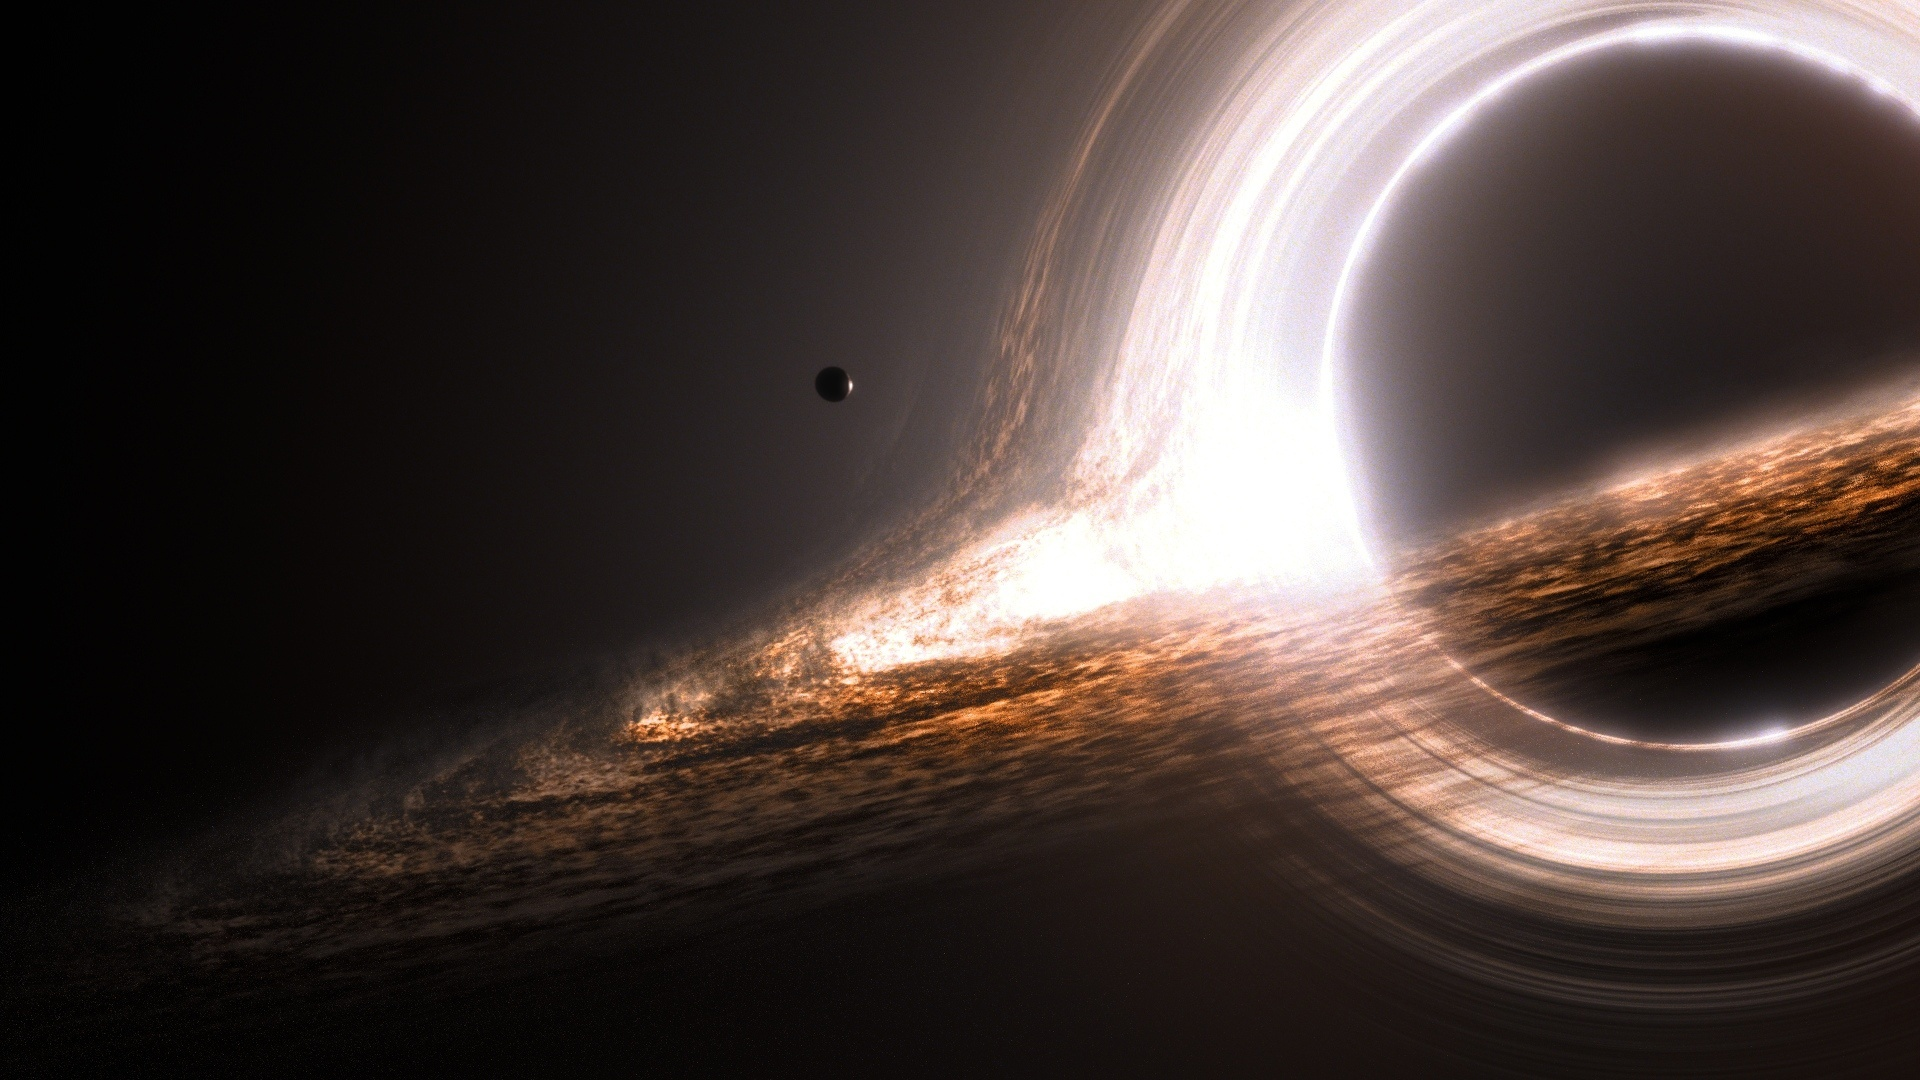
\includegraphics[height=\paperheight]{images/interstellar}}
\frame{\vspace*{12em}\titlepage}}
\frame{\tableofcontents}

\section{Erinnerungen}

\subsection{Gewöhnliche Turingmaschinen}

\begin{frame}{Ein Hoch auf Turingmaschinen}
  \begin{center}
    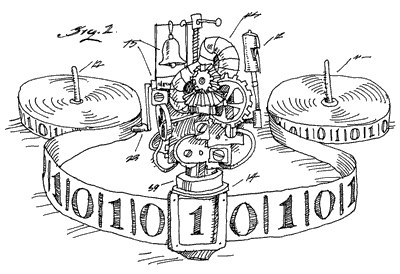
\includegraphics[width=0.6\textwidth]{images/turing-machine}
  \end{center}

  \begin{multicols}{2}
    \begin{enumerate}
      \item Schlichtheit
      \item Mechanischer Bezug
      \item Robustheit des Konzepts
      \item Äquivalenz zu anderen Modellen
      \item Querverbindungen
    \end{enumerate}
  \end{multicols}
\end{frame}
% mündlich: Es gibt Turingmaschinen mit 2 Zuständen und 4 Symbolen
% sowie mit 3 Zuständen und 3 Symbolen, deren Halteverhalten unbekannt ist.

\begin{frame}{Lustiges zu Turingmaschinen}
  \begin{enumerate}
    \item Schon kleine Turingmaschinen sind diffizil.
    \item Es gibt Turingmaschinen, deren Halteverhalten unabhängig von
    Standard-Axiomen der Mathematik ist.
    % Zum Beispiel: die TM, die nach einem Widerspruch in ZFC sucht.
    % Wenn ZFC konsistent ist, dann hält diese nicht.
    % Dieser Umstand ist aber nicht in ZFC beweisbar (Gödel II).
    \pause

    \item Alle sinnvollen Modelle für Berechenbarkeit stimmen für
    Funktionen~$\NN \to \NN$ überein.
    % Aber nicht für Funktionen höherer Ordnung!
    \pause

    \item Eine Menge ist genau dann rekursiv aufzählbar, wenn
    sie durch eine~$\Sigma_1$-Aussage definierbar ist:
    \[ \{ n \in \NN \,|\, \text{es gibt $m \in \NN$ mit $\heartsuit$} \}, \]
    \pause
    und wenn sie diophantisch ist:
    \[ \{ n \in \NN \,|\, \text{die Gl. $f(n,x_1,\ldots,x_m) = 0$
    besitzt eine Lösung} \}, \]
    wobei $f$ ein Polynom mit ganzzahligen Koeffizienten ist.
  \end{enumerate}
\end{frame}

\note{\justifying
  Eine~$\Sigma_1$-Aussage ist eine Aussage der Form
  \[ \text{"`Es gibt~$m \in \NN$ mit $\heartsuit$."',} \]
  wobei in der Teilaussage~$\heartsuit$ nur noch \emph{beschränkte
  Quantifikation} vorkommen darf -- also Formeln wie
  \[ \text{"`Für alle Zahlen kleiner als~$\cdots$ gilt \ldots"'} \]
  oder
  \[ \text{"`Es gibt eine Zahl kleiner als~$\cdots$ mit \ldots"'} \]
  und nicht Formeln wie
  \[ \text{"`Für alle Zahlen gilt \ldots"'} \]
  und
  \[ \text{"`Es gibt eine Zahl mit \ldots"'}. \]
  Die Teilaussage~$\heartsuit$ muss also in endlicher Zeit überprüfbar sein.\par
}


\subsection{Ordinalzahlen}

\begin{frame}{Ordinalzahlen messen Anordnung}
  \begin{center}
    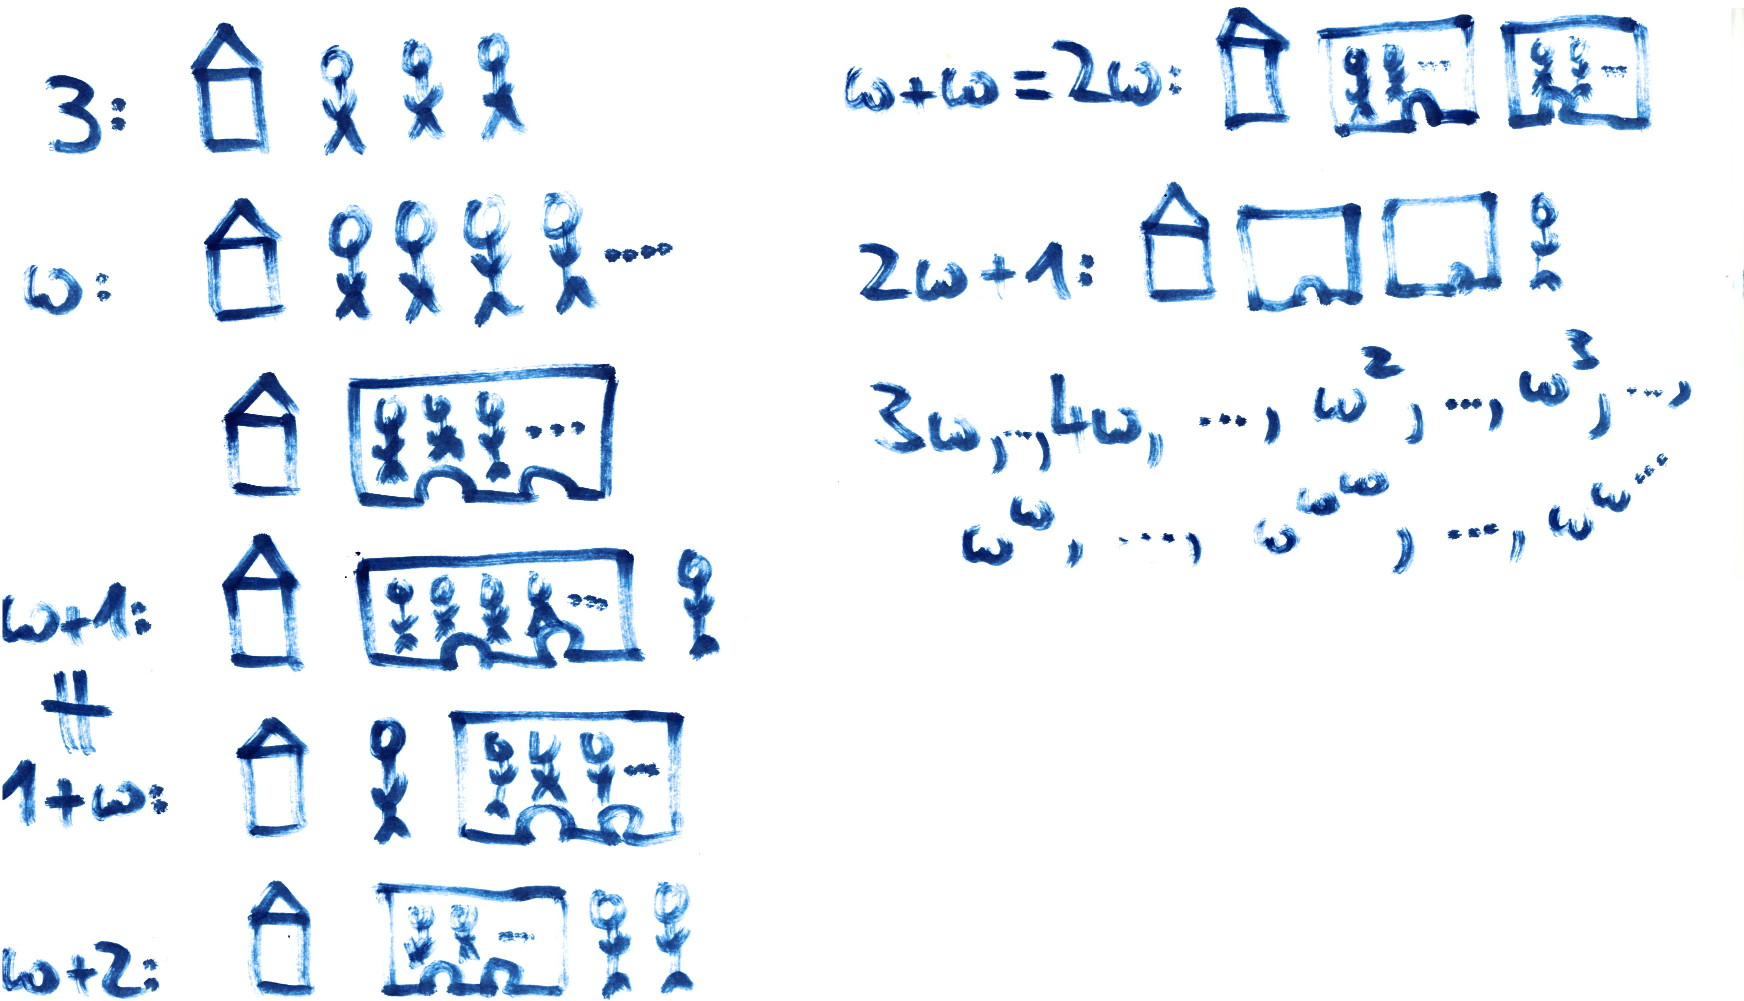
\includegraphics[width=\textwidth]{images/ordinal-intuition}
  \end{center}
\end{frame}

\note{\centering
  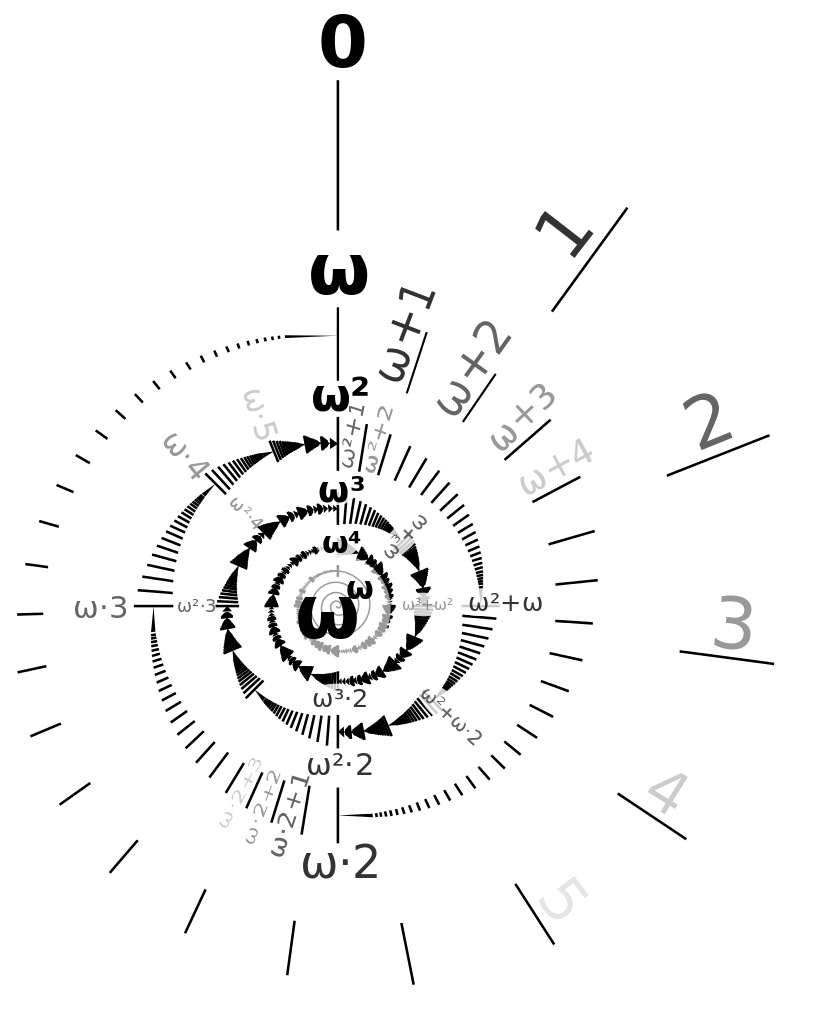
\includegraphics[width=0.7\textwidth]{images/ordinal-omega-omega}
  \par
}

\begin{frame}{Kardinalzahlen messen Anzahl}
  \begin{center}
    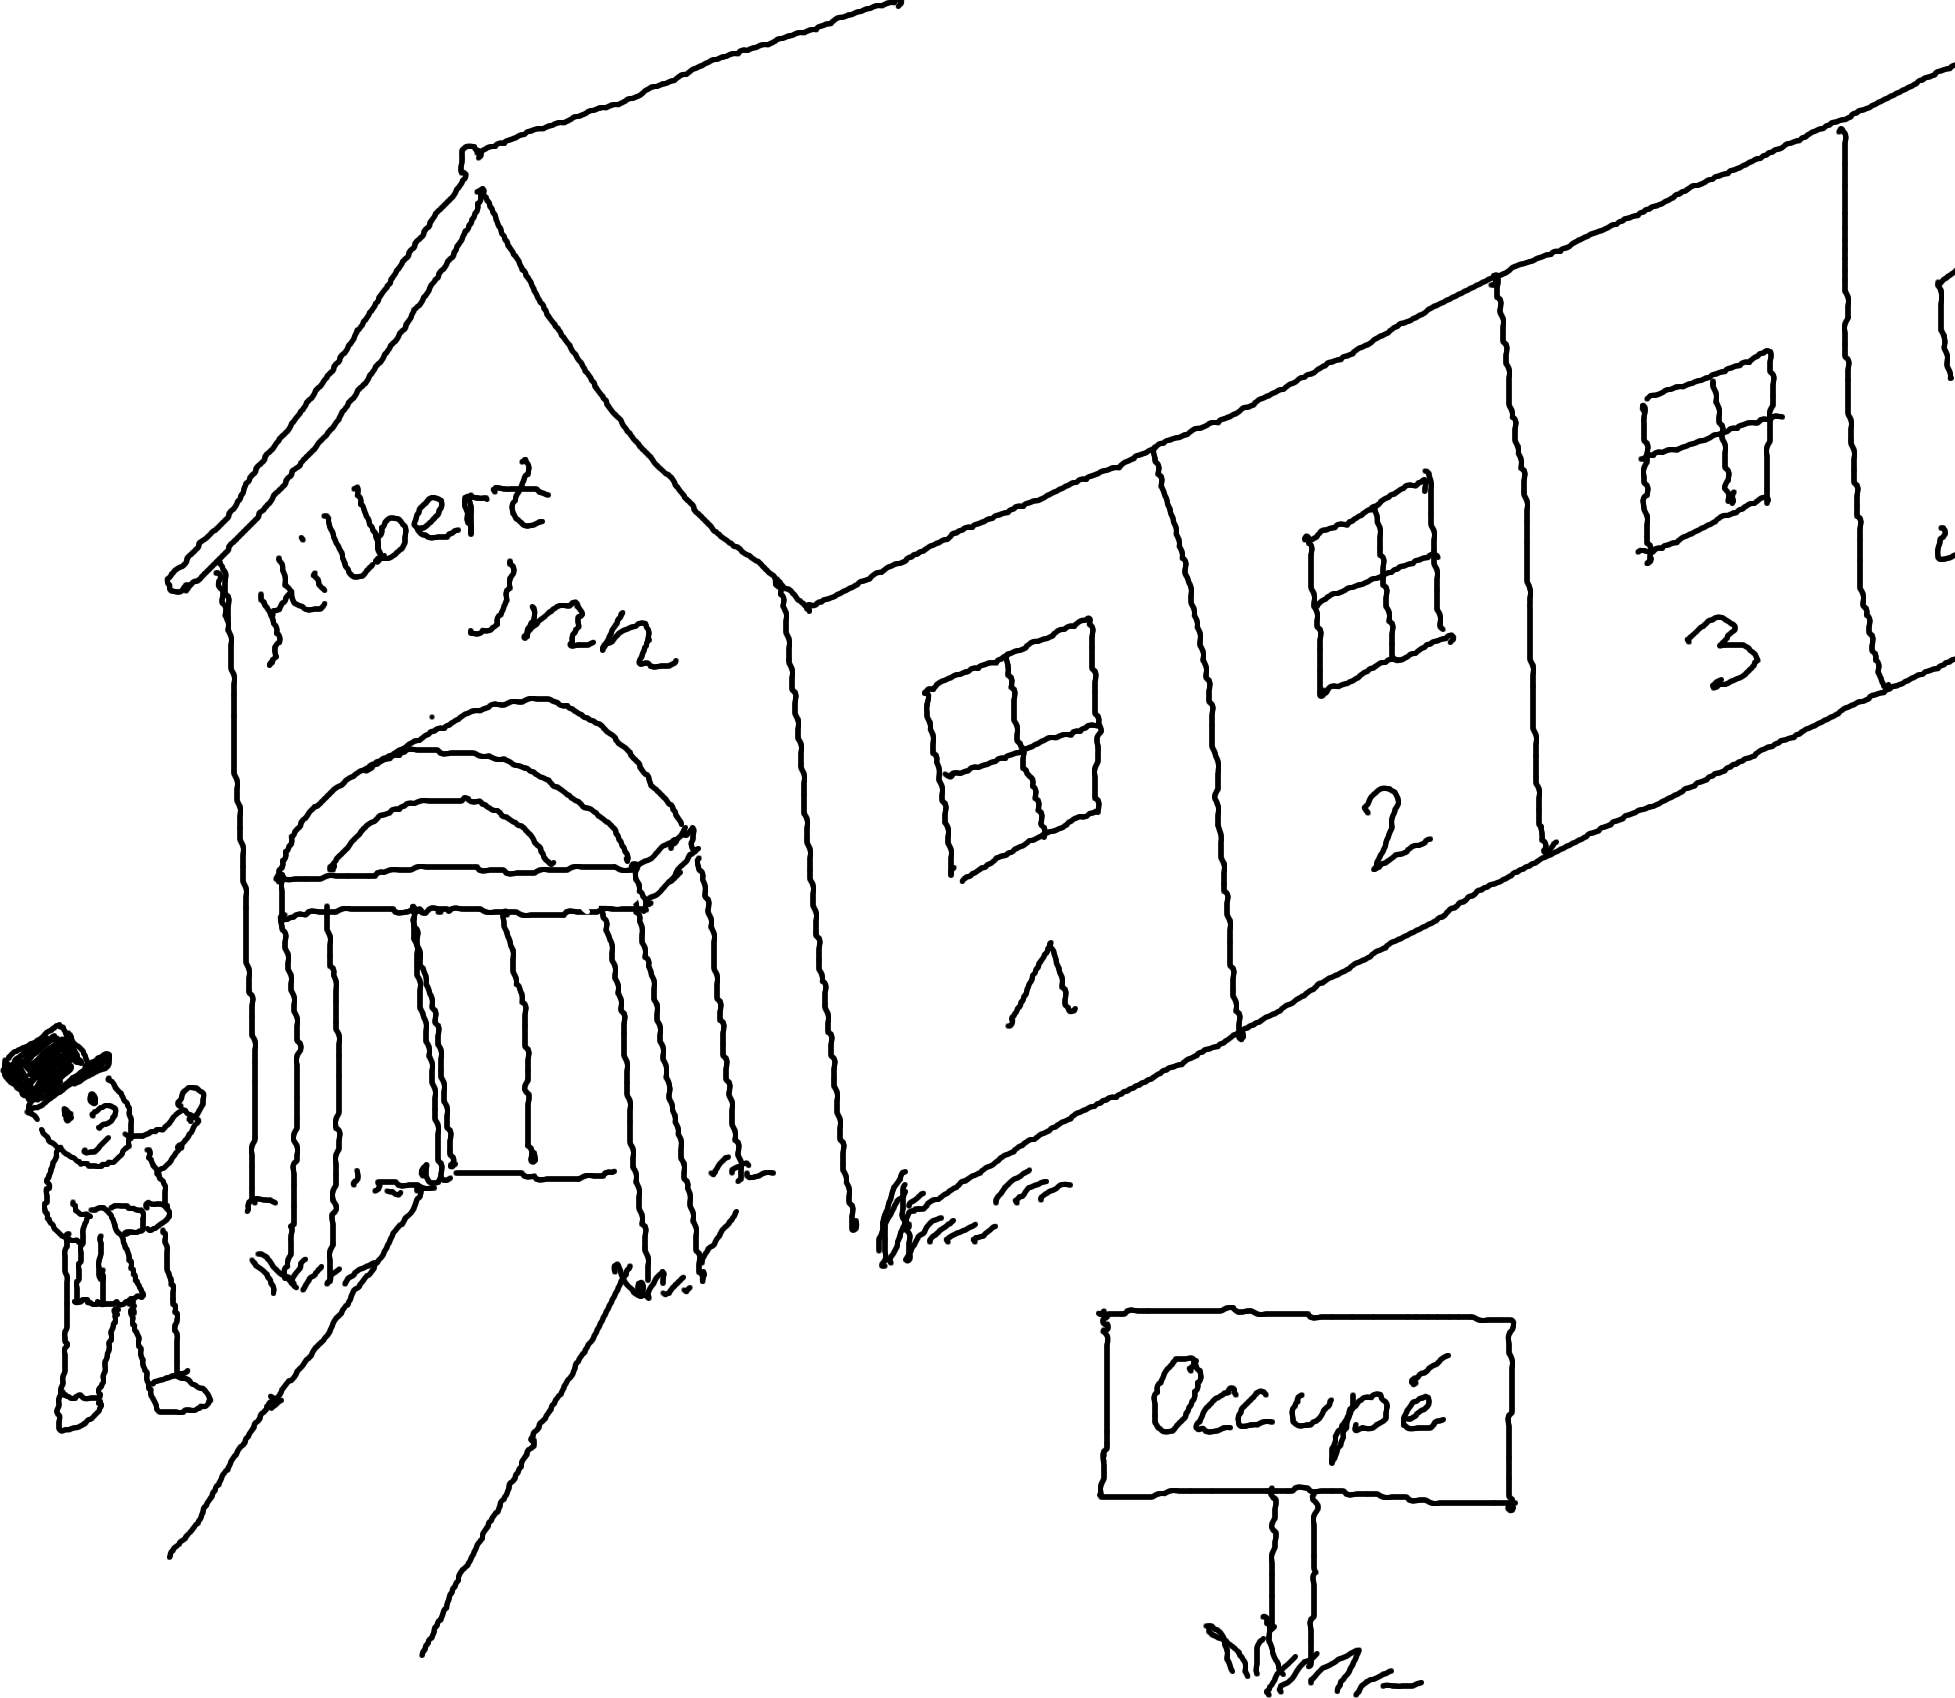
\includegraphics[width=0.5\textwidth]{images/hilberts-hotel}
  \end{center}

  \begin{itemize}
    \item Es gibt~$\aleph_0$ viele natürliche Zahlen.
    \pause
    \item $\aleph_0 + 1 = \aleph_0$, \quad
    \pause
    $\aleph_0 + \aleph_0 = \aleph_0$, \quad
    \pause
    $\aleph_0 \cdot \aleph_0 = \aleph_0$.
    \pause
    \item Es gibt mehr als~$\aleph_0$ viele reelle Zahlen.
  \end{itemize}
\end{frame}


\section[Grundlagen]{Grundlagen zu Superturingmaschinen}

\subsection{Erste Schritte}

\begin{frame}{Was sind Superturingmaschinen?}
  Bei Superturingmaschinen ist die Zeitachse spannender:
  \begin{itemize}
    \item normal: $0,\ 1,\ 2,\ \ldots$
    \item super:\phantom{rl} $0,\ 1,\ 2,\ \ldots,\ \omega,\ \omega + 1,\ \ldots,\ 2\omega,\ 2\omega
    + 1,\ \makebox[\widthof{R}][l]{$\ldots\ldots\ldots\ldots\ldots\ldots$}$
  \end{itemize}
  \bigskip

  Wird eine Limesordinalzahl erreicht, so wird
  \begin{itemize}
    \item die Maschine in einen designierten Zustand versetzt,
    \item der Schreib-/Lesekopf auf den Anfang bewegt und
    \item der "`lim sup"' aller vorherigen Bandinhalte genommen.
  \end{itemize}

  \begin{center}
    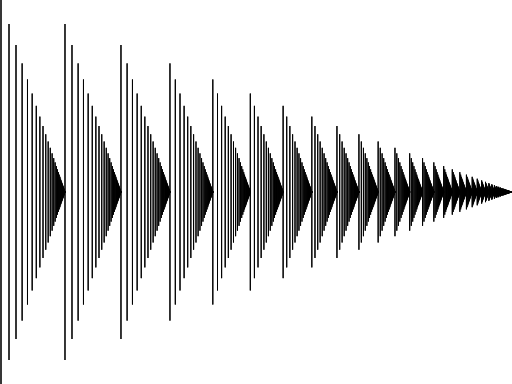
\includegraphics[width=0.35\textwidth]{images/ordinal-omega-squared}
  \end{center}
\end{frame}


\subsection[Fähigkeiten]{Fähigkeiten von Superturingmaschinen}

\begin{frame}{Was können Superturingmaschinen?}
  \begin{itemize}
    \item Alles, was gewöhnliche Turingmaschinen können.
    \item Zahlentheoretische Behauptungen überprüfen:
      \begin{itemize}
        \item $\forall$ -- "`Für alle Zahlen gilt \ldots"'    % omega
        \item $\exists$ -- "`Es gibt eine Zahl mit \ldots"'   % omega
        \item $\forall\,\exists$ -- "`Für alle Zahlen~$n$
        gibt es jeweils eine Zahl~$m$ mit \ldots"'            % 2 omega
        \item $\exists\,\forall$ -- "`Es gibt eine Zahl~$n$,
        sodass für alle Zahlen~$m$ gilt: \ldots"'             % omega
        \item $\forall\,\exists\,\forall$,                    % omega^2
        $\exists\,\forall\,\exists$, \ldots
      \end{itemize}
    \item Entscheiden, ob gewöhnliche Turingmaschinen halten.
    \item \ \\[-1.2em]\mbox{Superturingmaschinen und verwandte Maschinen simulieren.}
    \item $\Pi_1^1$- und $\Sigma_1^1$-Aussagen entscheiden.
  \end{itemize}
  \pause

  \hil{Aber:} Superturingmaschinen können nicht alle Funktionen berechnen
  und nicht jede 0/1-Folge aufs Band schreiben.
  % Es gibt~$2^{\aleph_0}$ viele Funktionen $\NN \to \NN$, aber nur $\aleph_0$
  % viele Superturingmaschinen.
\end{frame}

\begin{frame}{Fundierung von Bäumen}
  Ein Baum ist genau dann \hil{fundiert}, wenn er keinen unendlichen Pfad enthält.

  \begin{center}
    \scalebox{0.4}{\input{images/nonwellfounded-tree.pdf_t}}
  \end{center}

  Superturingmaschinen können die Fundiertheit von Bäumen entscheiden.
\end{frame}

\begin{frame}{Ein kleines Wunder}
  Superturingmaschinen können~$\Pi_1^1$- und $\Sigma_1^1$-Aussagen entscheiden:
  \[ \text{"`Für jede Funktion~$\NN \to \NN$ gilt \ldots"'} \]
  \[ \text{"`Es gibt eine Funktion~$\NN \to \NN$ mit \ldots"'} \]

  \vspace*{0.5em}
  Und das, obwohl es überabzählbar viele Funktionen~$\NN \to \NN$ gibt, aber
  Superturingmaschinen nur ein abzählbares Band verwenden und (nächste
  Folie) immer schon nach abzählbar vielen Schritten halten
  oder in Endlosschleifen geraten.
\end{frame}


\subsection[Laufzeit]{Laufzeit von Superturingmaschinen}

\begin{frame}{Wann halten Superturingmaschinen?}
  Schon nach \hil{abzählbar vielen} ($\leq \aleph_0$ vielen) Schritten hält jede
  Superturingmaschine entweder an oder wiederholt sich.
  \bigskip
  \pause

  \emph{Sprechweise.} Eine Ordinalzahl ist genau dann \hil{abzählbar}, wenn sie
  nur abzählbar viele Vorgänger hat.
  \bigskip

  Genau die abzählbaren Ordinalzahlen lassen sich in~$\RR$ einbetten.

  \begin{center}
    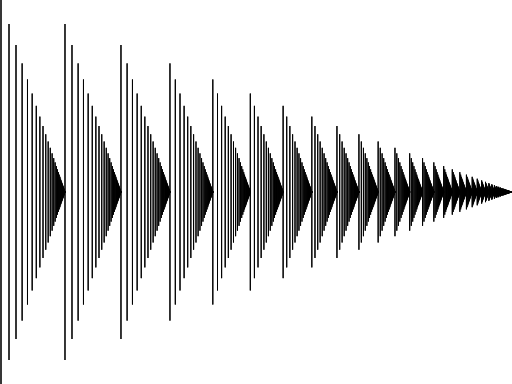
\includegraphics[width=0.35\textwidth]{images/ordinal-omega-squared}
  \end{center}
\end{frame}

\note{
  \emph{Notation.} Es ist~$\omega_1$ die erste Ordinalzahl, vor der
  \emph{überabzählbar} unendlich viele Ordinalzahlen kommen.
  \bigskip

  \emph{Behauptung.}
  Hat eine Superturingmaschine nach \emph{abzählbar vielen} Schritten noch
  nicht angehalten, so hält sie nie.
  \bigskip

  \justifying
  \emph{Beweis.} Angenommen, eine Superturingmaschine hat vor
  Schritt~$\omega_1$ noch nicht gehalten. Dann gibt es eine
  Ordinalzahl~$\alpha_0 < \omega_1$, zu der sich alle Zellen, die sich bis
  vor~$\omega_1$ stabilisieren werden, schon stabilisiert haben. Ferner gibt es
  Ordinalzahlen
  \[ \alpha_0 < \alpha_1 < \alpha_2 < \cdots < \omega_1, \]
  sodass sich zwischen~$\alpha_n$ und~$\alpha_{n+1}$ all die Zellen, die sich
  bis~$\omega_1$ noch ändern werden, jeweils mindestens einmal ändern.
  Sei~$\delta = \lim_{n \to \infty} \alpha_n$. Das ist eine Ordinalzahl~$<
  \omega_1$, also eine abzählbare Ordinalzahl. Dann ist die Aufnahme der
  Superturingmaschine bei~$\delta$ gleich der bei~$\omega_1$. Die
  Superturingmaschine wiederholt sich also.
  \par
}


\section{Besondere Phänomene}

\subsection[Wiederholungen]{Ausbrechen aus Wiederholungen}

\begin{frame}{Ausbrechen aus Wiederholungen}
  Was macht folgende Superturingmaschine?

  \code{Prüfe im Start- und Limeszustand, ob die aktuelle Zelle eine Eins enthält.
  \begin{itemize}
    \item Wenn ja, dann halte.
    \item Wenn nein, dann lass die Zelle aufleuchten und laufe ohne Unterlass nach
    rechts.
  \end{itemize}}
  \pause

  Sie scheint sich zu wiederholen, hält aber nach Schritt~$\omega^2$.
  \bigskip
  \pause

  Eine Superturingmaschine wiederholt sich genau dann, wenn
  \begin{itemize}
    \item die Aufnahmen zu zwei
    Limesordinalzeiten gleich sind und
    \item zwischen diesen Zeiten keine Zellen, die
    Null waren, zu Eins werden.
  \end{itemize}
\end{frame}


\subsection{Stempelbare Ordinalzahlen}

\begin{frame}{Stempelbare Ordinalzahlen}
  Eine Ordinalzahl~$\alpha$ ist genau dann \hil{stempelbar} (clockable),
  falls es eine Superturingmaschine gibt, die genau nach Schritt~$\alpha$ hält.

  \only<1>{\begin{itemize}
    \item Jede endliche Ordinalzahl ist stempelbar.
    \item Stempelbar sind außerdem: $\omega$, $2\omega$, $\omega^2$
    \item Sind~$\alpha$ und~$\beta$ stempelbar, so auch~$\alpha+\beta$
    und~$\alpha \cdot \beta$.
    \item Nur abzählbar viele Ordinalzahlen sind stempelbar.
    \item Jede rekursive Ordinalzahl ist stempelbar.
  \end{itemize}}

  \only<2>{
    \begin{block}{Beschleunigungssatz}
    Ist~$\alpha + n$ stempelbar, so auch~$\alpha$.
    \end{block}

    \begin{block}{Große-Lücken-Satz}
    Für jede stempelbare Ordinalzahl~$\alpha$
    gibt es eine Lücke der Länge~$\geq \alpha$ in den stempelbaren Ordinalzahlen.
    \end{block}

    \begin{block}{Viele-Lücken-Satz}
    Ist~$\alpha$ eine schreibbare Ordinalzahl,
    so gibt es mindestens~$\alpha$ viele Lücken der Länge~$\geq \alpha$ in den
    stempelbaren Ordinalzahlen.
    \end{block}
    % Lückenlose-Blöcke-Satz?
  }
\end{frame}

\note{\justifying
  Kurioserweise gibt es auch den \emph{Lückenlose-Blöcke-Satz} (Gapless Blocks
  Theorem): Es gibt in den Ordinalzahlen "`lange Abschnitte"' von lauter
  stempelbaren Ordinalzahlen.
  \par
}

\begin{frame}{Erinnerung: Diagonalisierung}
  \begin{center}
    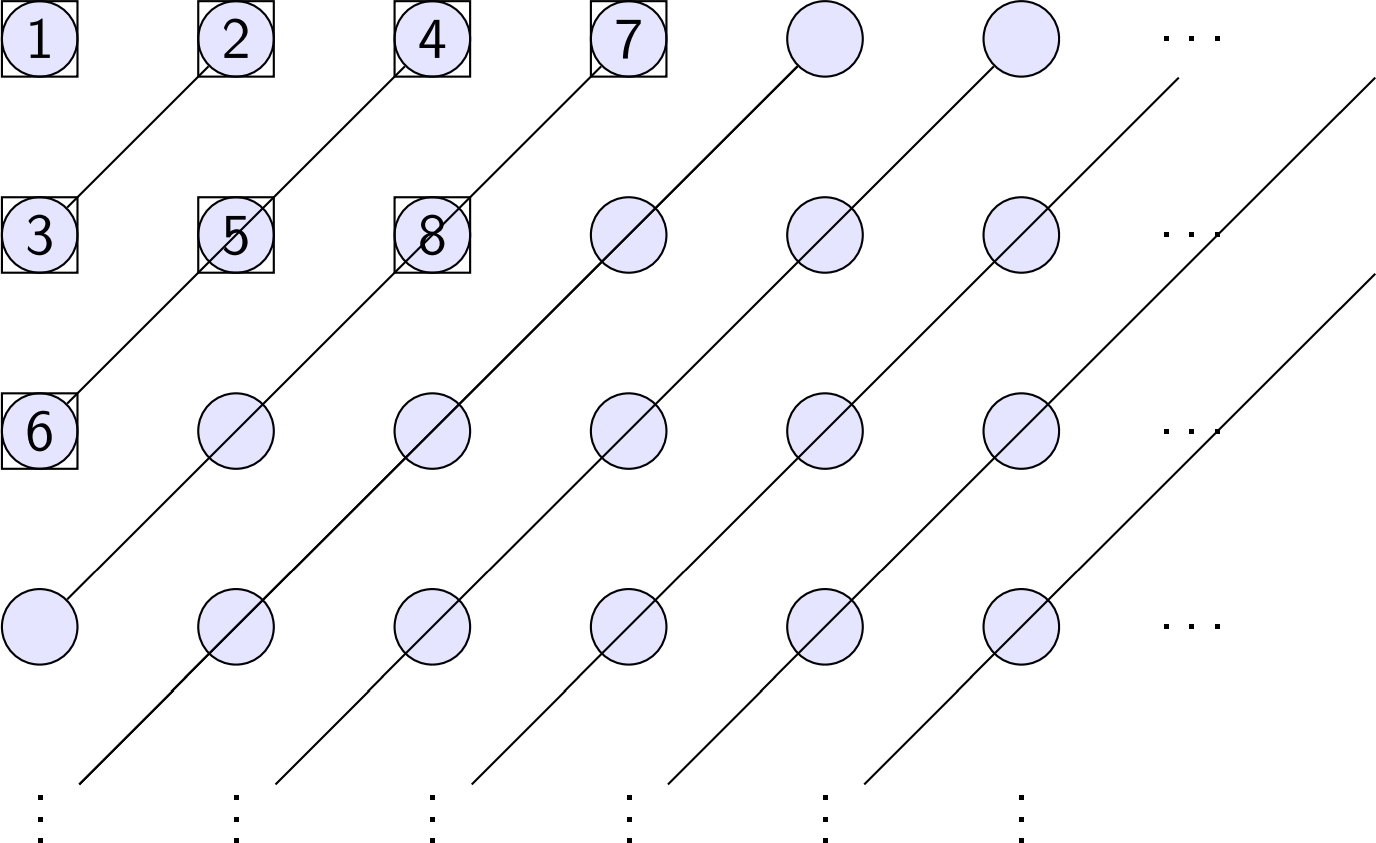
\includegraphics[width=0.8\textwidth]{images/diagonalization}
  \end{center}
\end{frame}

\begin{frame}{Lückenexistenzsatz}
  \mbox{Die erste Lücke nach jeder stempelbaren Ordinalzahl hat
  Länge~$\omega$.}
  \bigskip

  \vspace*{-1.2em}
  \justifying
  \emph{Beweis.} Sei~$\alpha$ eine stempelbare Ordinalzahl.
  Sei~$\beta$ die kleinste nicht-stempelbare Ordinalzahl nach~$\alpha$.
  Dann gibt es keine stempelbaren Ordinalzahlen zwischen~$\beta$ und~$\beta +
  \omega$. Und~$\beta + \omega$ selbst ist stempelbar durch folgendes Programm:
  \code{
    Simuliere alle Superturingmaschinen auf verzahnte Art und Weise.
    Behalte dabei insbesondere das Programm im Auge, das nach Schritt~$\alpha$
    halten wird. Sobald dieses gehalten hat, simuliere so lange weiter, bis der
    Zeitpunkt~$\beta$ erreicht ist, zu dem keine Superturingmaschine hält, und halte
    dann.}
  Zur Erkennung waren aber noch~$\omega$ Schritte nötig.
\end{frame}


\subsection{Lost-Melody-Theorem}

\begin{frame}{Lost-Melody-Theorem}
  Es gibt Bandinhalte, die
  \begin{itemize}
    \item Superturingmaschinen nicht schreiben, aber
    \item erkennen können.
  \end{itemize}
  \pause
  \bigskip

  \emph{Beweis.} Sei~$c$ eine Kodierung aller Ablauf{}folgen aller
  Superturingmaschinen als unendliche 0/1-Folge.
  \begin{itemize}
    \item Dann ist~$c$ nicht schreibbar.
    \item Aber~$c$ ist erkennbar.
  \end{itemize}

  \hfill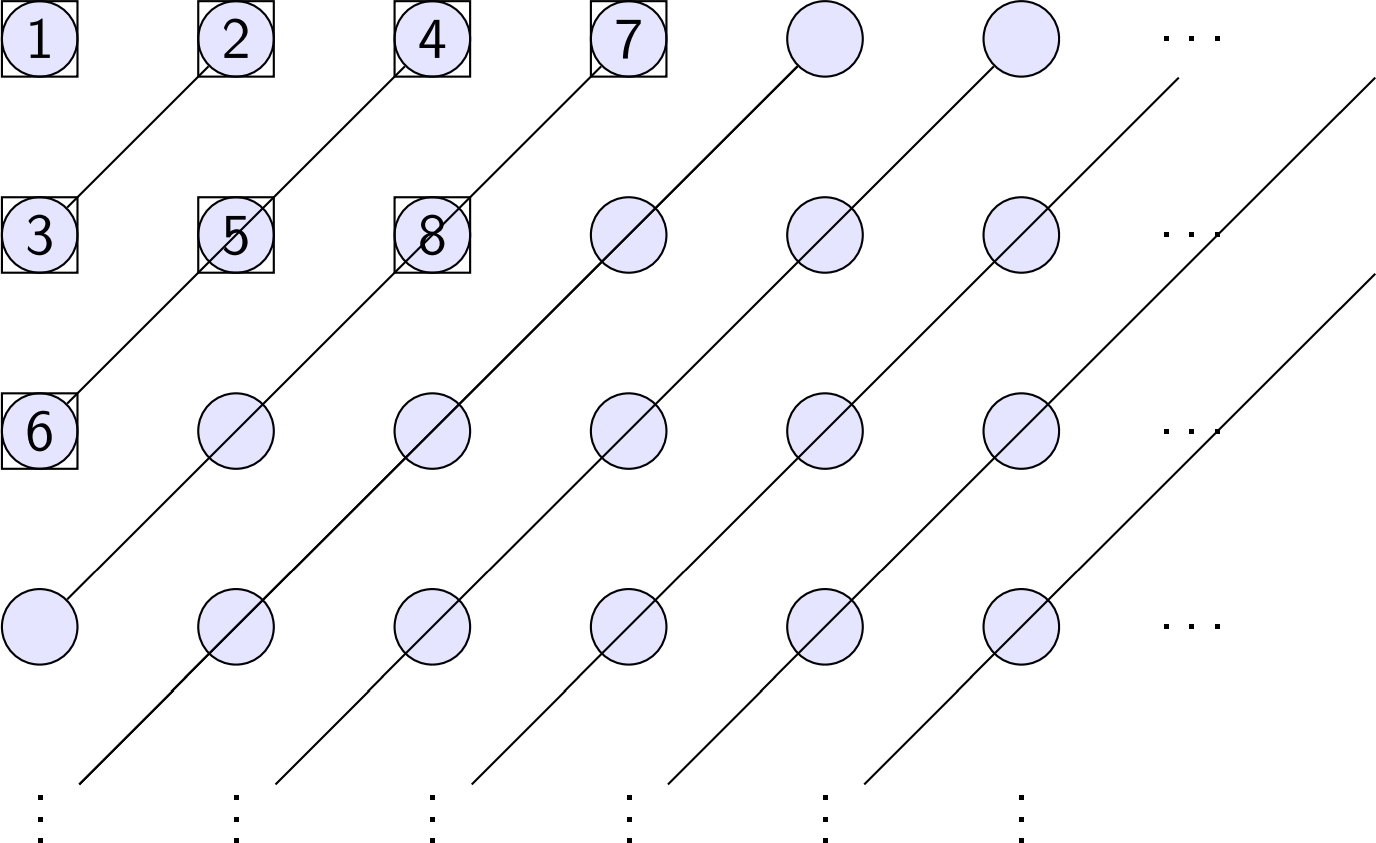
\includegraphics[width=0.4\textwidth]{images/diagonalization}
\end{frame}


\section[Effektive Topoi]{Der effektive Topos}

\subsection[Alternativuniversen]{Mathematische Alternativuniversen}

\begin{frame}{Mathematische Alternativuniversen}
  \justifying
  Zu jedem Rechenmodell~$\M$ gibt es einen
  \hil{Topos}~$\Eff(\M)$, in den wir mit \hil{Realisierbarkeitstheorie}
  hineinschauen können.
  \bigskip
  \pause

  \explanation{$\Eff(\TM) \models \text{"`Für jede Zahl~$n$ gibt es eine
  Primzahl~$p > n$."'}$}{Es gibt eine Turingmaschine, die eine Zahl~$n$ vom Band einliest
  und eine Primzahl~$p > n$ als Ausgabe aufs Band schreibt.}
  \bigskip

  \explanation{$\Eff(\TM) \models \text{"`Jede Zahl besitzt eine
  Primfaktorzerlegung."'}$}{Es gibt eine Turingmaschine, die eine Zahl~$n$ vom
  Band einliest und eine Liste von Primzahlen, deren Produkt~$n$ ist, aufs Band
  schreibt.}
\end{frame}

\note{\justifying
  Wenn man ganz normal Mathematik betreibt, so arbeitet man im "`Topos der
  Mengen"'. Es gibt aber auch andere mathematische Universen neben diesem. In
  diesen anderen Topoi gelten teilweise leicht andere logische Gesetze als die
  uns vertrauten; somit sieht die mathematische Landschaft in manchen Topoi
  etwas anders aus als die bekannte Landschaft im Topos der Mengen.
  \bigskip

  Jede geometrische Form (jeder topologischer Raum, jeder "`Situs"') gibt
  Anlass zu jeweils einem Topos (den "`Topos der Garben über der Form"');
  die entstehenden Topoi heißen "`Grothendieck-Topoi"', da es Grothendieck war,
  der dieses Konzept in den 1960er Jahren einführte. Topoi anderer Art sind die
  effektiven Topoi, die es für jeden Rechenmodell gibt: gewöhnliche
  Turingmaschinen ($\TM$), Superturingmaschinen ($\STM$), untypisiertes
  $\lambda$-Kalkül ($\lambdaC$), Maschinen in
  der realen Welt ($\RW$), \ldots\par
  \bigskip

  Neben der logischen Sicht gibt es auch eine geometrische Sicht auf Topoi:
  Topoi kann man sich als verallgemeinerte Arten von Räumen vorstellen. Etwa
  gibt es das Konzept des \emph{Punkts} eines Topos, das von offenen,
  abgeschlossenen und dichten \emph{Untertopoi} und das von stetigen
  Abbildungen zwischen Topoi.\par
}


\subsection[Intuitionistische Logik]{Das Wunder intuitionistischer Logik}

\begin{frame}{Was gilt in Alternativuniversen?}
  \hil{Metatheorem:} Jede Aussage, die sich \hil{intuitionistisch} beweisen
  lässt, gilt in allen Topoi.
  \bigskip

  {\centering
  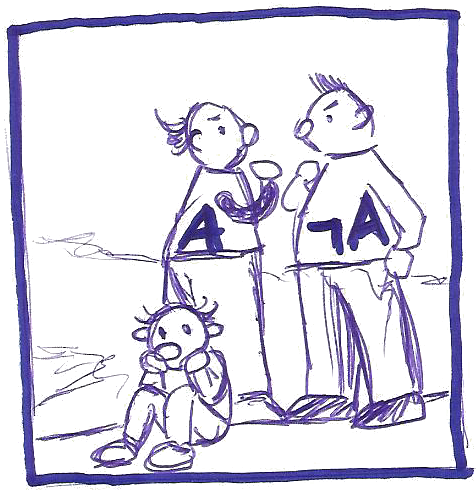
\includegraphics[width=0.2\textwidth]{images/lem}
  \par}

  \begin{block}{Schon gewusst?}
    Intuitionistische Logik ist wie klassische Logik, nur ohne:
    \begin{itemize}
      \item Axiom vom ausgeschlossenen Dritten (LEM): $\varphi \vee \neg\varphi$
      \item Axiom der Doppelnegationselimination (DNE): $\neg\neg\varphi \Rightarrow \varphi$
    \end{itemize}
    So sind Widerspruchsbeweise nicht pauschal möglich.
  \end{block}
\end{frame}

\begin{frame}{Wertschätzung intuitionistischer Logik}
  Der Verzicht aufs Axiom vom ausgeschlossenen Dritten erscheint zunächst
  schade, ist es doch ein gelegentlich hilfreiches Axiom. Allerdings:

  \begin{itemize}\justifying
    \item Man benötigt das Axiom seltener, als man vielleicht denkt.
    \item Der Verzicht ist gut für die mentale Hygiene.
    \item Mit intuitionistischer Logik kann man feinere Unterschiede abbilden.
    \item Aus intuitionistischen Beweisen kann man stets Programme extrahieren,
    die die bewiesenen Behauptungen bezeugen.
    \item \hil{Der Verzicht auf LEM ermöglicht die Hinzunahme
    kurioser unkonventioneller Axiome.}
  \end{itemize}
\end{frame}

\note{\justifying
  In klassischer Logik ist man gewohnt, doppelte Verneinungen sofort
  wegzustreichen. Da das in intuitionistischer Logik nicht möglich ist, muss
  man etwas mehr sprachliche Sorgfalt walten lassen. Insbesondere muss man
  zwischen echten Widerspruchsbeweisen und Beweisen von negierten Aussagen
  unterscheiden, in denen ebenfalls das Wort "`Widerspruch"' vorkommt:

  \begin{itemize}
  \item\justifying
  \emph{Beweis einer negierten Aussage (intuitionistisch zulässig):}
  Wir möchten~$\neg\psi$ zeigen. Angenommen, die Aussage~$\psi$ würde stimmen.
  Dann \ldots, das wäre ein Widerspruch. Somit~$\neg\psi$.

  In intuitionistischer Logik (wie auch in klassischer Logik) ist~$\neg\psi$
  nämlich als die Implikation $(\psi \Rightarrow \bot)$ definiert.

  \item \emph{Beweis durch Widerspruch (intuitionistisch nicht pauschal
  möglich):} Angenommen, die zu zeigende Aussage~$\varphi$ wäre falsch. Dann
  \ldots, das wäre ein Widerspruch. Somit ist~$\varphi$ wahr.

  Das intuitionistisch zulässige Teil in diesem Argument zeigt nur,
  dass~$\varphi$ \emph{nicht nicht} gilt: $\neg\neg\varphi$.\par
  \end{itemize}
}

\note{\justifying
  Vor ein paar Jahren tauchte ein Video von Kate Moss auf, das sie beim
  Konsumieren von Drogen zeigte. Aus dem Video war klar, dass es sich dabei entweder um
  Drogen von einem gewissen Typ~$A$ oder von einem gewissen Typ~$B$ handelte;
  aber es gab keinen direkten Beleg für einen der beiden Typen.
  Kate Moss wurde nicht verfolgt; in diesem Sinn verwendete das Justizsystem
  also intuitionistische Logik. Siehe
  \href{http://blog.sigfpe.com/2008/06/drugs-kate-moss-and-intuitionistic.html}{ein
  Blog-Post von Dan Piponi} über das Thema.
  \bigskip

  Intuitionistische Logik kann feinere Unterschiede abbilden als klassische Logik.
  Wenn wir zum Beispiel wissen, dass sich unser Haustürschlüssel irgendwo in
  der Wohnung befinden muss (da wir ihn letzte Nacht verwendet haben, um die Tür
  aufzusperren), wir ihn momentan aber nicht finden, so können wir intuitionistisch
  nicht die Aussage vertreten, dass es eine Stelle gäbe, an der der Schlüssel
  liege. Denn dazu müssten wir in der Lage sein, einen expliziten Zeugen dieser
  Existenzbehauptung (also den Aufenthaltsort des Schlüssels) anzugeben.
  Wir können intuitionistisch nur die durch doppelte Negation abgeschwächte Aussage
  vertreten.
  (Die Beispiele hinken etwas, da sie sich auf den Kenntnisstand von gewissen
  Personen beziehen.)
  \par
}

\note{\justifying
  Nebenbei bemerkt: Intuitionistische Mathematikerinnen behaupten \emph{nicht}, dass
  das Axiom vom ausgeschlossenen Dritten falsch sei (d.\,h. dass seine Negation
  gelten würde). Sie setzen es nur nicht in seiner vollen Allgemeinheit voraus.
  \bigskip

  Tatsächlich lassen sich manche Instanzen des Axioms auch intuitionistisch zeigen:
  Zum Beispiel folgt mit Induktion, dass jede natürliche Zahl gleich Null oder
  ungleich Null ist.
  \bigskip

  Die analoge Behauptung für reelle Zahlen lässt sich intuitionistisch nicht
  zeigen. Das hat eine Parallele in der Programmierung: Bekanntlich ist es
  unschicklich, Fließkommazahlen auf Gleichheit zu testen, während das bei
  Ganzzahlen kein Problem ist. Das wird auf einer späteren Folie noch näher
  ausgeführt.
  \par
}

\note{\justifying
  Eine letzte Bemerkung. Philosophinnen untersuchen nicht nur was \emph{wahr}
  ist, sondern auch was stimmen \emph{sollte}, was \emph{möglich} ist, was
  \emph{notwendig} ist, was jemand \emph{weiß} oder was jemand \emph{glaubt}.
  Das formalisiert man mit \emph{modalen Operatoren}.
  \bigskip

  Als Mathematikerin kann man daher manchmal neidisch werden. In
  intuitionistischer Logik aber gibt es durchaus auch eine Vielzahl von modalen
  Operatoren! Die Doppelnegation ist das wichtigste Beispiel.\par
}


\subsection[Tautologien]{Effektive Bedeutung klassischer Tautologien}

\begin{frame}{LEM für Gleichheit von Funktionen}
  \explanationspoiler{$\Eff(\TM) \models \begin{minipage}[t]{0.7\textwidth}
  "`Für jede Funktion~$f : \NN \to \NN$ gilt: Entweder ist~$f$ die Nullfunktion
  oder nicht."'\end{minipage}$}{Es gibt eine Turingmaschine, die eine Kodierung
  einer Turingmaschine~$M$, welche eine Funktion $\NN \to \NN$ berechnet, als
  Eingabe vom Band liest und dann entscheidet, ob~$M$ stets Null als Ausgabe
  produziert oder nicht.}{Das stimmt nicht.}
  \bigskip
  \pause

  \emph{Bemerkung:} Aus externer Sicht ist das Objekt~$\NN^\NN$ des effektiven
  Topos die Menge der \hil{berechenbaren} Funktionen~$\NN \to \NN$.
  \bigskip
  \pause

  In~$\Eff(\STM)$ stimmt die Aussage.
\end{frame}

\begin{frame}{LEM fürs Halten von Turingmaschinen}
  \explanationspoiler{$\Eff(\TM) \models \text{"`Jede Turingmaschine~$M$ hält
  oder hält nicht."'}$}{Es gibt eine Turingmaschine, die die Kodierung einer
  Turingmaschine~$M$ als Eingabe vom Band liest und dann entscheidet, ob~$M$
  hält oder nicht.}{Das stimmt nicht.}
  \bigskip
  \pause

  In~$\Eff(\STM)$ stimmt die Aussage.
\end{frame}

\begin{frame}{LEM für Gleichheit reeller Zahlen}
  \justifying
  Die Aussage
  \[ \text{"`Jede reelle Zahl ist Null oder ungleich Null."'} \]
  ist in intuitionistischer Logik äquivalent zu
  \[ \text{"`Jede Turingmaschine hält oder hält nicht."'}, \]
  gilt also nicht in~$\Eff(\TM)$, aber in~$\Eff(\STM)$.
  \bigskip

  Denn zu einer Turingmaschine~$M$ kann man die reelle Zahl~$0{,}000\ldots$
  betrachten, deren~$n$-te Nachkommastelle genau dann eine~$1$ ist, wenn~$M$
  nach Schritt~$n$ hält, und sonst~$0$ ist.
  \bigskip

  Umgekehrt kann man zu einer reellen Zahl~$x$ diejenige Turingmaschine
  betrachten, die die Nachkommaziffern von~$x$ nach einer von Null
  verschiedenen Ziffer absucht und genau dann hält, wenn sie eine solche Ziffer
  gefunden hat.\par
\end{frame}

\note{\justifying
  Stimmt die Aussage in~$\Eff(\RW)$, dem effektiven Topos zu Maschinen der
  realen Welt? Das heißt: Ist es möglich, in der realen Welt ein Halteorakel zu
  bauen? Also eine Maschine, welche die Beschreibung einer Turingmaschine einliest
  und dann korrekt ausgibt, ob die Turingmaschine hält oder nicht?
  \bigskip

  Da es hier nicht um das Halteproblem für Maschinen der realen Welt geht
  (welches für Maschinen der realen Welt wegen des üblichen Arguments nicht
  entscheidbar ist), sondern nur um das Halteproblem für Turingmaschinen, ist
  die Antwort "`ja"' nicht prinzipiell ausgeschlossen. Vielleicht sind Tricks
  mit schwarzen Löchern und relativistischer Zeitdilatation möglich.
  \par
}

\begin{frame}{Markovs Prinzip}
  \explanationspoiler{$\Eff(\TM) \models \begin{minipage}[t]{0.7\textwidth}
  "`Für jede Funktion~$f : \NN \to \NN$, welche nicht die Nullfunktion ist,
  gibt es eine Stelle~$n \in \NN$ mit~$f(n) \neq 0$."'\end{minipage}$}{Es gibt
  eine Turingmaschine, die eine Kodierung einer Turingmaschine~$M$, welche eine
  Funktion $\NN \to \NN$ und zwar nicht die Nullfunktion berechnet, als Eingabe
  vom Band liest und dann eine Zahl~$n$ aufs Band schreibt, sodass~$M$ bei
  Eingabe von~$n$ nicht Null aufs Band schreibt.}{Das stimmt! (Unbeschränkte
  Suche.)}
\end{frame}

\begin{frame}{Das Auswahlaxiom}
  \justifying
  Eine Menge~$X$ ist genau dann \hil{projektiv}, wenn für jede Menge~$Y$ und
  jede Aussage~$\varphi(x,y)$ mit Parametern~$x \in X$, $y \in Y$ gilt:
  \begin{center}\parbox{0.86\textwidth}{
    Wenn es zu jedem~$x \in X$ ein~$y \in Y$ mit~$\varphi(x,y)$ gibt,
    so gibt es eine Abbildung~$f : X \to Y$ mit~$\varphi(x,f(x))$ für alle~$x \in X$.
  }\end{center}
  % \[ \forall x \in X\_ \exists y \in Y\_ \varphi(x,y) \ \Longrightarrow\
  %   \exists f : X \to Y\_ \forall x \in X\_ \varphi(x,f(x)) \]
  Das \hil{Auswahlaxiom} klassischer Mathematik besagt, dass dort jede Menge
  projektiv ist.

  \begin{itemize}
    \item In~$\Eff(\TM)$ ist~$\NN$ projektiv,~$\NN^\NN$ aber nicht.
    \item In~$\Eff(\STM)$ sind~$\NN$ und~$\NN^\NN$ projektiv.
    \item In~$\Eff(\RW)$ ist~$\NN^\NN$ projektiv, falls Blackboxes möglich
    sind.
  \end{itemize}
\end{frame}

\note{\justifying
  Auch intuitionistisch ist jede endliche Menge projektiv. Der Beweis, dass~$X =
  \{ 1, \ldots, n \}$ projektiv ist, geht so: Nach Voraussetzung existiert
  für jede Zahl~$i = 1,\ldots,n$ je mindestens ein Element~$y_i \in Y$
  mit~$\varphi(i, y_i)$. Also ist~$f : X \to Y$ mit~$i \mapsto y_i$ eine
  Abbildung der gewünschten Art.
  \bigskip

  Der Beweis lässt sich allerdings nicht auf den Fall übertragen, dass die
  Menge~$X$ unendlich groß ist. Der Grund dafür ist etwas subtil. Es hängt
  damit zusammen, dass Beweise nicht unendlich lang sein dürfen und dass in
  einem Geltungsbereich (Scope) nur endlich viele Variablen vorkommen
  dürfen.\par
}

\note{\justifying
  Dass die Aussage des Auswahlaxioms nicht trivial ist, zeigt sich,
  wenn man die Aussage~"`$\NN^\NN$ ist projektiv"' in~$\Eff(\TM)$
  interpretiert. Aus
  \begin{center}\parbox{0.86\textwidth}{
    Es gibt eine Turingmaschine~$M$, die die Kodierung einer
    Turingmaschine~$P$, welche eine Funktion~$f : \NN \to \NN$ berechnet, vom Band
    einliest und die Kodierung eines Elements~$M(P) \in Y$ zusammen mit einem
    Zeugen von~$\varphi(f,M(P))$ ausgibt.
  }\end{center}
  folgt nämlich nicht, dass:
  \begin{center}\parbox{0.86\textwidth}{
    Es gibt eine berechenbare Abbildung~$g$ von der Menge der berechenbaren
    Funktionen~$f : \NN \to \NN$ in die Menge~$Y$ sodass für alle solche
    Funktionen~$f$ in~$\Eff(\TM)$ gilt, dass~$\varphi(f,g(f))$.
  }\end{center}
  Man könnte denken, dass die gesuchte berechenbare Abbildung~$g$ einfach
  von~$M$ berechnet wird. Aber das stimmt im Allgemeinen nicht. Denn ist~$f :
  \NN \to \NN$ eine durch eine Turingmaschine~$P$ berechenbare Funktion, so
  hängt das Element~$M(P)$ im Allgemeinen von der konkreten Umsetzung von~$f$
  durch~$P$ ab. Verschiedene Umsetzungen können verschiedene Elemente geben.
  Bei einer Abbildung, wie es~$g$ werden soll, darf das nicht sein.\par
}

\note{\justifying
  Man kann zeigen (schöne Übungsaufgabe): In~$\Eff(\M)$ ist eine Assembly~$X$
  genau dann projektiv, wenn es eine~$\M$-Maschine~$A$ gibt, die kanonische
  Darstellungen für alle Elemente von~$X$ berechnet: Ist~$r$ eine Kodierung
  eines Elements~$x$ von~$X$, so ist auch~$A(r)$ eine Kodierung von~$x$; und
  ist~$s$ eine weitere Kodierung von~$x$, so ist~$A(r) = A(s)$.

  \begin{itemize}
    \item\justifying Für~$X = \NN^\NN$ aus~$\Eff(\TM)$ gibt es keine solche Maschine.
    \item Für~$X = \NN^\NN$ aus~$\Eff(\STM)$ gibt es eine solche Maschine:
    Lese die Kodierung einer Superturingmaschine~$R$, welche eine Funktion~$f :
    \NN \to \NN$ berechnet, vom Band ein. Simuliere dann auf verzahnte Art und
    Weise alle Superturingmaschinen. Sobald eine gefunden ist, deren
    Ausgabeverhalten dem von~$R$ gleicht, stoppe und gebe die Kodierung der
    gefundenen Superturingmaschine aus.
    \item Für~$X = \NN^\NN$ aus~$\Eff(\RW)$ gibt es eine solche Maschine, falls
    in der realen Welt Blackboxes möglich sind: Die gesucht Maschine nimmt eine
    Maschine der realen Welt entgegen und verpackt sie in eine Blackbox,
    sodass die Kommunikation mit der Maschine nur noch über ihr Interface
    möglich und ihre innere Funktionsweise unbeobachtbar ist.
  \end{itemize}
}

\begin{frame}{Church--Turing-These}
  \justifying
  Die \hil{Church--Turing-These} besagt: Lässt sich eine Funktion $f : \NN \to
  \NN$ in der "`realen Welt berechnen"', so gibt es eine Turingmaschine,
  die~$f$ berechnet.
  \bigskip

  \explanationspoiler{$\Eff(\TM) \models \begin{minipage}[t]{0.7\textwidth}
  "`Jede Funktion~$f : \NN \to \NN$ lässt sich durch eine Turingmaschine
  berechnen."'\end{minipage}$}{Es gibt eine Turingmaschine, die eine Kodierung
  einer Turingmaschine~$M$, welche eine Funktion~$f : \NN \to \NN$ berechnet, als
  Eingabe vom Band liest und dann die Kodierung einer Turingmaschine,
  welche~$f$ berechnet, aufs Band schreibt.}{Das ist trivial! "`cat"' ist die
  gesuchte Maschine.}
  \bigskip
  \pause

  In~$\Eff(\STM)$ und~$\Eff(\lambdaC)$ stimmt die Aussage nicht.
\end{frame}

\note{\justifying
  Der effektive Topos zu Turingmaschinen ist also eine schöne Umgebung für die
  Informatik, da in ihm \emph{jede Funktion~$\NN \to \NN$ berechenbar ist} und
  unberechenbare Funktionen aussortiert wurden.
  \bigskip

  Vielleicht vermutet man hierbei einen Widerspruch. Sind nicht etwa folgende
  Funktionen unberechenbar? Was verhindert ihre Existenz im effektiven Topos?
  \begin{align*}
    H(n) &= \begin{cases}
      1, & \text{falls die~$n$-te Turingmaschine hält,} \\
      0, & \text{sonst.}
    \end{cases} \\
    BB(n) &= \text{höchste Anzahl Schritte, die eine haltende Turingmaschine} \\
    &\qquad\quad \text{mit~$n$ Zuständen durchführt, bevor sie hält.}
  \end{align*}

  Um zu zeigen, dass~$H$ und~$BB$ beides totale Funktionen~$\NN \to \NN$ sind
  -- und nur auf solche bezieht sich die Church--Turing-These --, ist LEM nötig!
  Für~$H$, damit die Fallunterscheidung getroffen werden kann. Für~$BB$, weil
  implizit das Lemma verwendet wurde, dass eine subendliche Menge natürlicher
  Zahlen ein größtes Element enthält.\par
}

\note{\justifying
  Die Aussage, dass \emph{jede} Funktion~$\NN \to \NN$ durch eine
  Turingmaschine berechenbar ist, ist auch als \emph{formale
  Church--Turing-These} bekannt.
  \begin{itemize}
    \item\justifying In~$\Eff(\STM)$ gilt sie nicht, denn aus einer
    Superturingmaschine, welche eine Funktion~$\NN \to \NN$ berechnet, kann man
    nur in den seltensten Fällen in eine gewöhnliche Turingmaschine mit
    demselben Ausgabeverhalten umwandeln.
    \item In~$\Eff(\lambdaC)$ gilt die formale Church--Turing-These ebenfalls
    nicht, aber aus einem anderen Grund. Die These lautet in diesem Fall:
    \begin{center}\parbox{0.83\textwidth}{
      Es gibt einen~$\lambda$-Term~$T$, sodass für jeden~$\lambda$-Term~$u$,
      welcher eine Funktion~$f : \NN \to \NN$ berechnet, der~$\lambda$-Term~$T\ u$
      die Kodierung einer Turingmaschine ist, welche~$f$ berechnet.
    }\end{center}
    Der ominöse Term~$T$ kann sein Argument~$u$ nur auf Eingaben auswerten, er
    hat aber keinen Zugriff auf die syntaktische Struktur von~$u$.
    (Konventionsgemäß werden in~$\Eff(\TM)$ Turingmaschinen höherer Ordnung
    dadurch realisiert, dass sie als Argument Kodierungen von
    Turingmaschinen erhalten. Beim~$\lambda$-Kalkül ist der Umweg über
    syntaktische Kodierungen nicht nötig und wird in~$\Eff(\lambdaC)$ auch
    nicht verfolgt.)
  \end{itemize}
}

% \begin{document}

\begin{frame}{Automatische Stetigkeit}
  \justifying
  Im üblichen Universum stimmt folgende Aussage \hil{nicht}:
  \[ \text{"`Jede Funktion~$f : \RR \to \RR$ ist stetig."'} \]
  Eine Funktion~$f$ heißt genau dann \hil{stetig}, falls für jede Zahl~$x$ zur
  Bestimmung von endlich vielen Nachkomma\-stel\-len von~$f(x)$ schon
  endlich viele Nachkommastellen von~$x$ genügen.\par

  \centering
  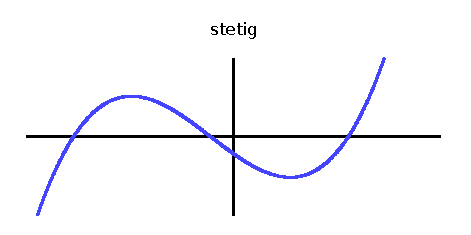
\includegraphics[width=0.5\textwidth]{images/plot-1}
  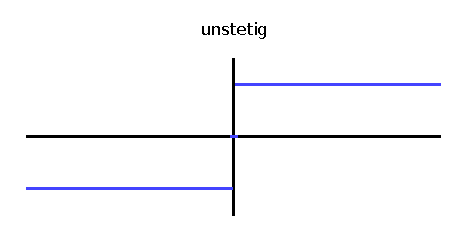
\includegraphics[width=0.5\textwidth]{images/plot-2}
  \par
  \pause

  \justifying
  Stimmt in~$\Eff(\TM)$. \pause
  Stimmt in~$\Eff(\RW)$, falls private Kommunikationskanäle
  möglich sind und in endlicher Zeit nur endlich viele Rechenschritte
  ausgeführt werden können.\par
\end{frame}

\note{\justifying
  Gibt es nicht offensichtlich unstetige Funktionen? Wie etwa die
  Signumfunktion?
  \[ \mathrm{sgn} : \RR \to \RR, \quad
    x \mapsto \begin{cases}
      -1, & \text{falls $x < 0$,} \\
      0,  & \text{falls $x = 0$,} \\
      1,  & \text{falls $x > 0$.}
    \end{cases}
  \]
  Ohne Verwendung von LEM ist die Situation nicht so trivial. Ohne es kann man
  nämlich nicht zeigen, dass diese Zuordnung eine auf ganz~$\RR$ definierte
  Funktion definiert: Dazu benötigte man das Lemma, dass jede reelle Zahl
  kleiner, gleich oder größer als Null ist. Dieses Lemma impliziert aber die
  schwächere Aussage, dass jede reelle Zahl gleich Null oder ungleich Null ist.
  Wir haben schon gesehen, dass diese Aussage in~$\Eff(\TM)$ nicht stimmt.
  \medskip

  Ohne LEM definiert obige Zuordnung nur eine Funktion~$M \to \RR$, wobei~$M =
  \{ x \in \RR \,|\, x < 0 \vee x = 0 \vee x > 0 \}$. Über solche Funktionen
  geht es hier aber nicht.
  \par
}

\note{\justifying
  Die in der Mathematik üblichen Definitionen des Konzepts reeller Zahlen sind
  in~$\Eff(\TM)$, $\Eff(\STM)$ und~$\Eff(\RW)$ alle zueinander äquivalent
  (obwohl sie es unter bloßer Verwendung von intuitionistischer Logik nicht
  sind).\bigskip

  Aus externer Sicht ist eine reelle Zahl in jedem der drei Fälle durch
  eine Maschine gegeben, die in sich konsistente, beliebig genaue
  Approximationen produziert. Etwa kann man eine solche Maschine nach
  Approximationen auf drei, sieben und zehn Ziffern fragen und die Antworten
  \[ 3.1417777777, \quad 3.1415926777 \quad\text{und}\quad 3.1415926535 \]
  erhalten.
  \bigskip

  Maschinen, welche andere, aber genauso gute Approximationen
  liefern, stellen dieselbe reelle Zahl dar.\par
}

\note{\justifying\footnotesize
  Die Aussage~"`Alle Funktionen~$\RR \to \RR$ sind stetig."' des effektiven
  Topos bedeutet: Es gibt eine Maschine~$M$, die
  \begin{enumerate}
    \item\justifying eine Maschine~$A$, welche eine Funktion~$f : \RR \to \RR$
    berechnet,
    \item eine Maschine~$X$, welche eine reelle Zahl~$x$ repräsentiert, sowie
    \item eine natürliche Zahl~$n$
  \end{enumerate}
  als Argumente nimmt und eine natürliche Zahl~$m$ mit folgender Eigenschaft
  ausgibt: Für jede reelle Zahl~$\tilde x$, deren erste~$m$ Ziffern mit denen
  von~$x$ übereinstimmen, stimmen die ersten~$n$ Ziffern von~$f(x)$ mit denen
  von~$f(\tilde x)$ überein.\smallskip

  Im Fall der realen Welt kann man wie folgt versuchen, eine derartige
  Maschine~$M$ zu konstruieren. Gegeben~$A$, $X$ und~$n$, wendet sie~$A$ auf
  eine leichte Variante~$X'$ von~$X$ an: Die Maschine~$X'$ soll dasselbe
  Ausgabeverhalten zeigen wie~$X$, allerdings bei jedem Aufruf über einen
  privaten Kommunikationskanal an~$M$ die Information übermitteln, wie viele
  Stellen abgefragt wurden. Da~$X'$ dasselbe Ausgabeverhalten wie~$X$ zeigt,
  muss~$A$ per Vertrag auf~$X'$ genauso reagieren wie auf~$X$.\smallskip

  Wenn nun in endlicher Zeit nur endlich viele Rechenschritte durchführbar sind, so
  muss~$M$ nur warten, bis~$A$ die Zahl~$f(x)$ auf~$n$ Stellen genau berechnet
  hat, und kann dann nachsehen, wie viele Stellen~$A$ für diese Berechnung
  benötigt hat. Für jede andere Zahl, die~$x$ in diesen Stellen gleicht,
  produziert somit~$A$ dieselben~$n$ Ziffern.\par
}

\note{\justifying
  Kein Fan von reellen Zahlen? Dasselbe Phänomen zeigt sich auch bei Funktionen
  von anderen Typen. Zum Beispiel für Funktionen~$f : \BB^\NN \to \BB$. Dabei
  ist~$\BB = \{ 0, 1 \}$ die Menge der Bools. Eine solche Funktion heißt genau
  dann \emph{stetig}, wenn es für jedes Argument~$x \in \BB^\NN$ (also jede
  Funktion~$x : \NN \to \BB$) eine natürliche Zahl~$m$ gibt, sodass~$f(x)$ nur
  von den ersten~$m$ Funktionswerten von~$x$ abhängt.\bigskip

  In~$\Eff(\TM)$ stimmt es, dass jede solche Funktion~$f$ stetig ist. Das ist
  der tiefere Grund dafür, wieso die "`scheinbar unmöglichen
  Haskell-Programme"' funktionieren.\par
}

\begin{frame}{Seltsame Größenverhältnisse}
  \only<1-2>{
    Es gibt keine Surjektion~$\NN \to \NN^\NN$; die Menge~$\NN^\NN$ der
    Funktionen~$\NN \to \NN$ ist viel größer als~$\NN$.
    \bigskip

    In klassischer Logik folgt: Es gibt auch keine Injektion~$\NN^\NN \to \NN$.
    Das drückt dieselbe Intuition über das Größenverhältnis aus.
    \bigskip

    {\centering
    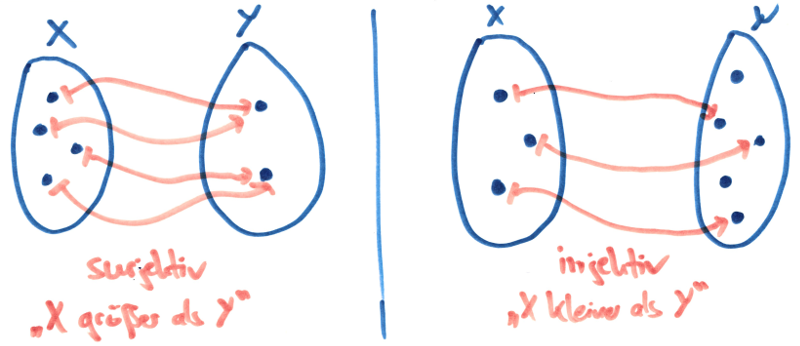
\includegraphics[width=0.8\textwidth]{images/groessenverhaeltnisse}
    \par}

    \pause
    Aber in~$\Eff(\STM)$ gibt es eine solche Injektion!
  }

  \only<3>{
    {\centering
    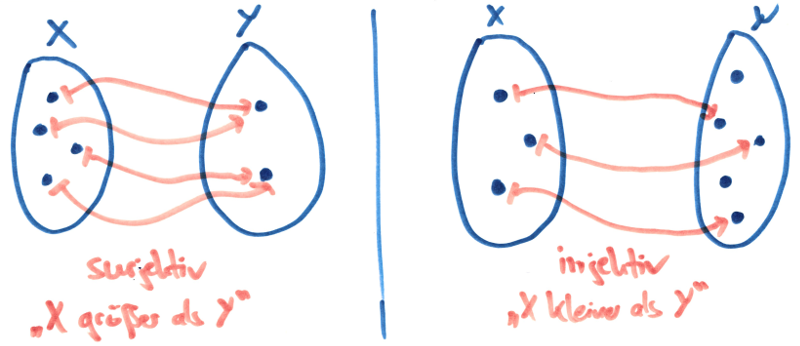
\includegraphics[width=0.7\textwidth]{images/groessenverhaeltnisse}
    \par}

    \explanation{$\Eff(\STM) \models \text{"`Es gibt eine Injektion~$\NN^\NN \to
    \NN$."'}$}{Es gibt eine Superturingmaschine, welche bei Eingabe einer
    Kodierung einer Superturingmaschine~$A$, welche eine Funktion~$\NN \to \NN$ berechnet,
    eine Zahl~$n(A)$ berechnet und aufs Band schreibt. Dabei darf nur dann~$n(A)
    = n(B)$ sein, wenn~$A$ und~$B$ dieselbe Funktion berechnen.}
  }

  \only<4>{
    \justifying
    Die Superturingmaschine
    \code{
      Lese die Kodierung einer Superturingmaschine~$A$ vom Band ein.
      Simuliere nun alle Superturingmaschinen auf verzahnte Art und Weise.
      Sobald eine gefunden ist, deren Ausgabeverhalten dem von~$A$ gleicht,
      höre auf und gebe die Nummer~$n$ dieser Maschine aus.
    }
    schreibt bei Eingabe einer Kodierung einer Superturingmaschine~$A$, welche
    eine Funktion~$\NN \to \NN$ berechnet, eine Zahl~$n(A)$ aufs Band. Dabei ist
    nur dann~$n(A) = n(B)$, wenn~$A$ und~$B$ dieselbe Funktion berechnen.
    \par
  }
\end{frame}

\note{\justifying
  Die von der beschriebenen Superturingmaschine ausgegebene Zahl~$n$ hängt vom
  Ausgabeverhalten von~$A$, der gewählten Reihenfolge aller
  Superturingmaschinen und von den Details der Verzahnung ab -- nicht aber von
  der Implementierung von~$A$.\medskip

  Die Suche terminiert, da es ja mindestens eine Superturingmaschine gibt, die
  bei Eingabe einer jeden natürlichen Zahl terminiert und dabei dasselbe
  Ausgabeverhalten wie~$A$ zeigt: $A$ selbst.\par
}

\note{\justifying
  Weil er so schön ist, hier der intuitionistisch zulässige Beweis, dass es
  keine Surjektion~$\NN \to \NN^\NN$ gibt:\bigskip

  Sei~$s : \NN \to \NN^\NN$ irgendeine Abbildung. Wir möchten nachweisen,
  dass~$s$ nicht surjektiv ist. Dazu betrachten wir die Abbildung~$f : \NN \to
  \NN$ mit
  \[ f(n) \vcentcolon= s(n)(n) + 1. \]
  Dieses Element~$f \in \NN^\NN$ kann von~$s$ nicht getroffen werden: Wenn es
  eine natürliche Zahl~$m$ mit~$s(m) = f$ gäbe, so wäre
  \[ s(m)(m) = f(m) = s(m)(m) + 1. \]
}

\note{\justifying
  Bei dieser Thematik ist es wichtig, nicht die externe und die interne Sicht
  durcheinanderzubringen. Sonst landet man bei \emph{Skolems Paradox}: Wie kann
  es sein, dass es in~$\Eff(\TM)$ keine Surjektion~$\NN \to \NN^\NN$ gibt, wo
  doch~$\NN^\NN$ nur berechenbare Funktionen enthält und es von diesen nur
  abzählbar viele gibt?\bigskip

  Die Auflösung ist: Es stimmt zwar, dass aus externer Sicht das
  Objekt~$\NN^\NN$ von~$\Eff(\TM)$, das ist aus externer Sicht die Menge der
  berechenbaren Funktionen~$\NN \to \NN$, abzählbar ist und dass es daher eine
  Surjektion (sogar Bijektion)~$\NN \to \NN^\NN$ gibt.\bigskip

  Diese Surjektion, und auch jede andere, ist aber entweder nicht berechenbar, daher
  nicht in~$\Eff(\TM)$ enthalten, oder zwar berechenbar, aber so beschaffen,
  dass es keinen berechenbaren Zeugen ihrer Surjektivität gibt. Daher
  sieht~$\NN^\NN$ aus der Sicht von~$\Eff(\TM)$ wie eine überabzählbare Menge
  aus, in Übereinstimmung mit Cantors intuitionistisch zulässigen Beweis.\par
}

\end{document}

Ein Hoch auf Turingmaschinen
* Einfachheit
* Maschinelle Umsetzung klar
* Robustheit des Konzepts
* Äquivalenz zu anderen Modellen (aber nur für N --> N)
* Verbindungen zur Logik
* (aber: "TM sind nicht alles", siehe zum Beispiel R-Maschinen oder QTM)

Crashkurs Ordinalzahlen

Erste Schritte mit Superturingmaschinen
* Definition
* Beispielaufgaben
* Halteproblem
* Schwerere Aufgaben

Besondere Phänomene
* Ausbrechen aus Wiederholungen
* Lost Melody
* Abmessbare Ordinalzahlen

Effektiver Topos

"Allgemein sollten im Vortrag auch Maschinen vorgeführt werden, deren
Halteverhalten von mengentheoretischen Eigenschaften abhängt. Zum Beispiel die
Sache mit der Unabhängigkeit von BB(n) für kleine Wert von n von Adam Yedidia
und Scott Aaronson. http://www.scottaaronson.com/busybeaver.pdf"
